\documentclass[lettersize,journal]{IEEEtran}
\usepackage{amsmath,amsfonts}
% \usepackage{algorithmic}
% \usepackage{algorithm}
\usepackage[linesnumbered, ruled]{algorithm2e}
\usepackage{array}
\usepackage[caption=false,font=normalsize,labelfont=sf,textfont=sf]{subfig}
\usepackage{textcomp}
\usepackage{stfloats}
\usepackage{url}
\usepackage{verbatim}
\usepackage{graphicx}
\usepackage{cite}
\hyphenation{op-tical net-works semi-conduc-tor IEEE-Xplore}
% updated with editorial comments 8/9/2021

\begin{document}

\title{{\huge CS303 Project 2 Report\\}{
Capacitated Arc Routing Problem (CARP) solver}}

\author{12111012 Kuang Liang}

\maketitle

\begin{abstract}
This document describes my work on CS303 project 2: CARP, containing the introduction of the problem, preliminaries of this report, the methods I used in the solver and the experiments I have done to test the solver. 
\end{abstract}

\section{Introduction}

\IEEEPARstart{C}{apacitated} Arc Routing Problem, CARP in short, is a classic NP-hard problem. CARP is one variant of Arc Routing Problem. The problem is modeled on a graph, where each edge has a cost and some has a demand. Out agent has limited capacity, so it must go back to the depot to empty it’s current load before it’s load is over it's capacity. The goal of the problem is to find a path with minimum total cost, on which the agent can satisfy all demands\cite{ref1}. This problem has a wide application in practice, like road planning for garbage transfer trucks.

In this project, I wrote a python program to generate a relatively optimal solution in limited time for an arbitrary CARP instance using genetic algorithm, and I will explain how it works and how it performs in this report.

\section{Preliminary}

\begin{center}
    \begin{tabular}{l|l}
        Symbol & Description \\ \hline\hline
        $P=(G,C,D,c,d)$ & the problem we want to solve \\
        $G=(V,E)$ & the graph of the problem \\
        $V$ & the vertex set of the graph \\
        $E$ & the edge set of the graph \\
        $e_i=(u_i,v_i)$ & an edge in the edge set \\
        $C$ & the capacity of the vehicle \\
        $D$ & the depot vertex \\
        $c$ & the cost function of edges \\
        $d$ & the demand function of edges \\
        $a$ & an arc in the graph or the solution \\
        $tc_a$ & the total cost of an arc \\
        $td_a$ & the total demand of an arc \\
        $s$ & a solution of the problem \\
        $tc_s$ & the total cost of a solution \\
        $dist(u,v)$ & the distance between two vertices \\
        $popsize$ & the size of the population \\
    \end{tabular}
\end{center}

CARP can be specified by a tuple $P=(G,C,D,c,d)$. $G=(V,E)$ is a undirected connected graph, $C\in\mathbf{R}^+$ is the capacity of the vehicle. $D\in V$ is the depot vertex. $c:E\to\mathbf{R}^+$ is the cost function which evaluates the cost of each edge. $d:E\to\mathbf{R}^+\cup\{0\}$ is the demand function which evaluates the demand of each edge, and $d(e_0)=0$ means the edge $e_0$ is not required (so the agent may not go through it). In this project, in order to ensure there is at least one solution, we assume that we have infinite number of vehicles, and $\forall e\in E,d(e)\leq C$.

An \textbf{arc} $a=(e_0,e_1,...,e_l)$ is a circuit begin from and end with $D$, which means $e_0=(D,v_0),e_l=(u_l,D)$ and $\forall0\leq i<l,e_i=(u_i,v_i),v_i=u_{i+1}$. The total cost of an arc $tc_a(a)=\sum_{e\in a}c(e)$ is the sum of the cost of the edges in it, and the total demand of an arc $td_a$ is the sum of the demand of the edges in it. An arc is \textbf{valid} if and only if $td_a(a)\leq C$. A \textbf{solution} $S=\{a_0,a_1,...\}$ is a multiset of several \textbf{valid} arcs, and the total cost of a solution $tc_s(s)=\sum_{a\in s}tc_a(a)$ is the sum of the cost of the arcs in it. A \textbf{valid} solution must contains all of required edges, which means $\forall e\in E(d(e)\not=0\to\exists a_0\in S(e\in a_0))$. Finally, our target is to find a valid solution with minimum total cost.

Note that we can pass an edge without dealing with its demand. In order to simplify our notations, we assume that if there is an edge $(u,v,c,d)$ in the graph where $d\not=0$, there is also an edge $(u,v,c,0)$ in the graph, which the agent can go through when it do not want to deal with the demand on the original edge. This will not change the time or space complexity of our algorithm but make the problem far easier to define.

\section{Methodology}

\subsection{General workflow}

Our method can be divided into four parts. First, we use \textbf{Floyd algorithm} to calculate the distance between every pair of vertices in the graph, because after choosing two demands $e_1,e_2$ to satisfy, it is always optimal for the agent to transform between $v_1$ and $u_2$ by the shortest path. Therefore, we only care about the order we deal with the demands in our algorithm, and \textbf{do not store other edges in our solution}. Second, we generate some solutions by some rules as the initial population. Third, we use some methods to mutate the population, and choose better individuals in it to be the next population. Finally, repeat the third step until time runs out, and output the solution.

\subsection{Part1. Floyd}

Floyd algorithm is a well known algorithm to calculate the distance (length of shortest path) of all the pairs of vertices in a graph in $O(|V|^3)$ time and $O(|V|^2)$ space, so I will not go into more detail here. Later, we will use $dist(u,v)$ to indicate the distance between $u$ and $v$, which we have already calculated in this part.

\subsection{Part2. Initialize population}

Basically, when generating an new individual, we just maintain a demand edge set, and choose a demand to put into the vehicle if it has enough capacity, or empty the vehicle at the depot vertex otherwise. However, instead of randomly choose a demand, some empirical laws can help us generate better individual that tends to optimize our final result:

\begin{itemize}
    \item [1.] Maximize the distance from the task to the depot;
    \item [2.] Minimize the distance from the task to the depot;
    \item [3.] Maximize the term $\frac{d(e)}{sc(e)}$;
    \item [4.] Minimize the term $\frac{d(e)}{sc(e)}$;
    \item [5.] Use rule \textbf{1.} if the vehicle is less than half-full, otherwise use \textbf{2.}\cite{ref3}.
\end{itemize}

$sc(e_i)=dist(p,u_i)$ is the serving cost of edge $e_i$ when the agent is at vertex $p$ now. With the $O(1)$ $dist$ function, we can choose a demand we want in $O(|E|)$ time under any rule. Here is the pseudo-code of generating a new individual in $O(|E|^2)$ time:

\begin{algorithm}
    \caption{Generate a new individual}
    \KwData{problem $P$, rule $r$}
    \KwResult{solution $s$}
    Initialize $s$ and $a$ to be empty\;
    $req=P$'s all required edges\;
    \For {$req\not=\emptyset$} {
        $e=$ the best demand edge in $req$ under rule $r$\;
        \eIf {$td_a(a+e)\leq C$} {
            $a=a+e$\;
            Remove $e$ from $req$\;
        } {
            $s=s+a$\;
            Empty $a$\;
        }
    }
    $s=s+a$\;
\end{algorithm}

Repeat it for a constant integer $popsize$ times with different rules, we will get an initial population. The total time complexity is $O(popsize\times|E|^2)$.

\subsection{Part3. Mutation}

In this part, we mutate our individuals in different ways, and select better ones from them to be the next generation:

\begin{itemize}
    \item [1.] \textbf{Flip}. Flip one edge in it.
    \item [2.] \textbf{Single Insertion}. Try to insert a demand to another position.
    \item [3.] \textbf{Double Insertion}. Try to insert two adjacent demands to another position.
    \item [4.] \textbf{Swap}. Swap two demands\cite{ref3}.
    \item [5.] \textbf{Single route optimization}. Reverse a segment of an arc, see \textbf{Figure1.(a)}.
    \item [6.] \textbf{2-OPT plan 1.} Break the arcs $a,b$ into $(a_1,a_2),(b_1,b_2)$, and combine $(a_1,b_2),(b_1,a_2)$ to be two new arcs, see \textbf{Figure 1.(b)}.
    \item [7.] \textbf{2-OPT plan 2.} Break the arcs $a,b$ into $(a_1,a_2),(b_1,b_2)$, and combine $(a_1,r(b_1)),(r(b_2),a_2)$ to be two new arcs, where $r$ means reversed, see \textbf{Figure 1.(c)}\cite{ref2}.
\end{itemize}

\begin{figure}
    \centering
    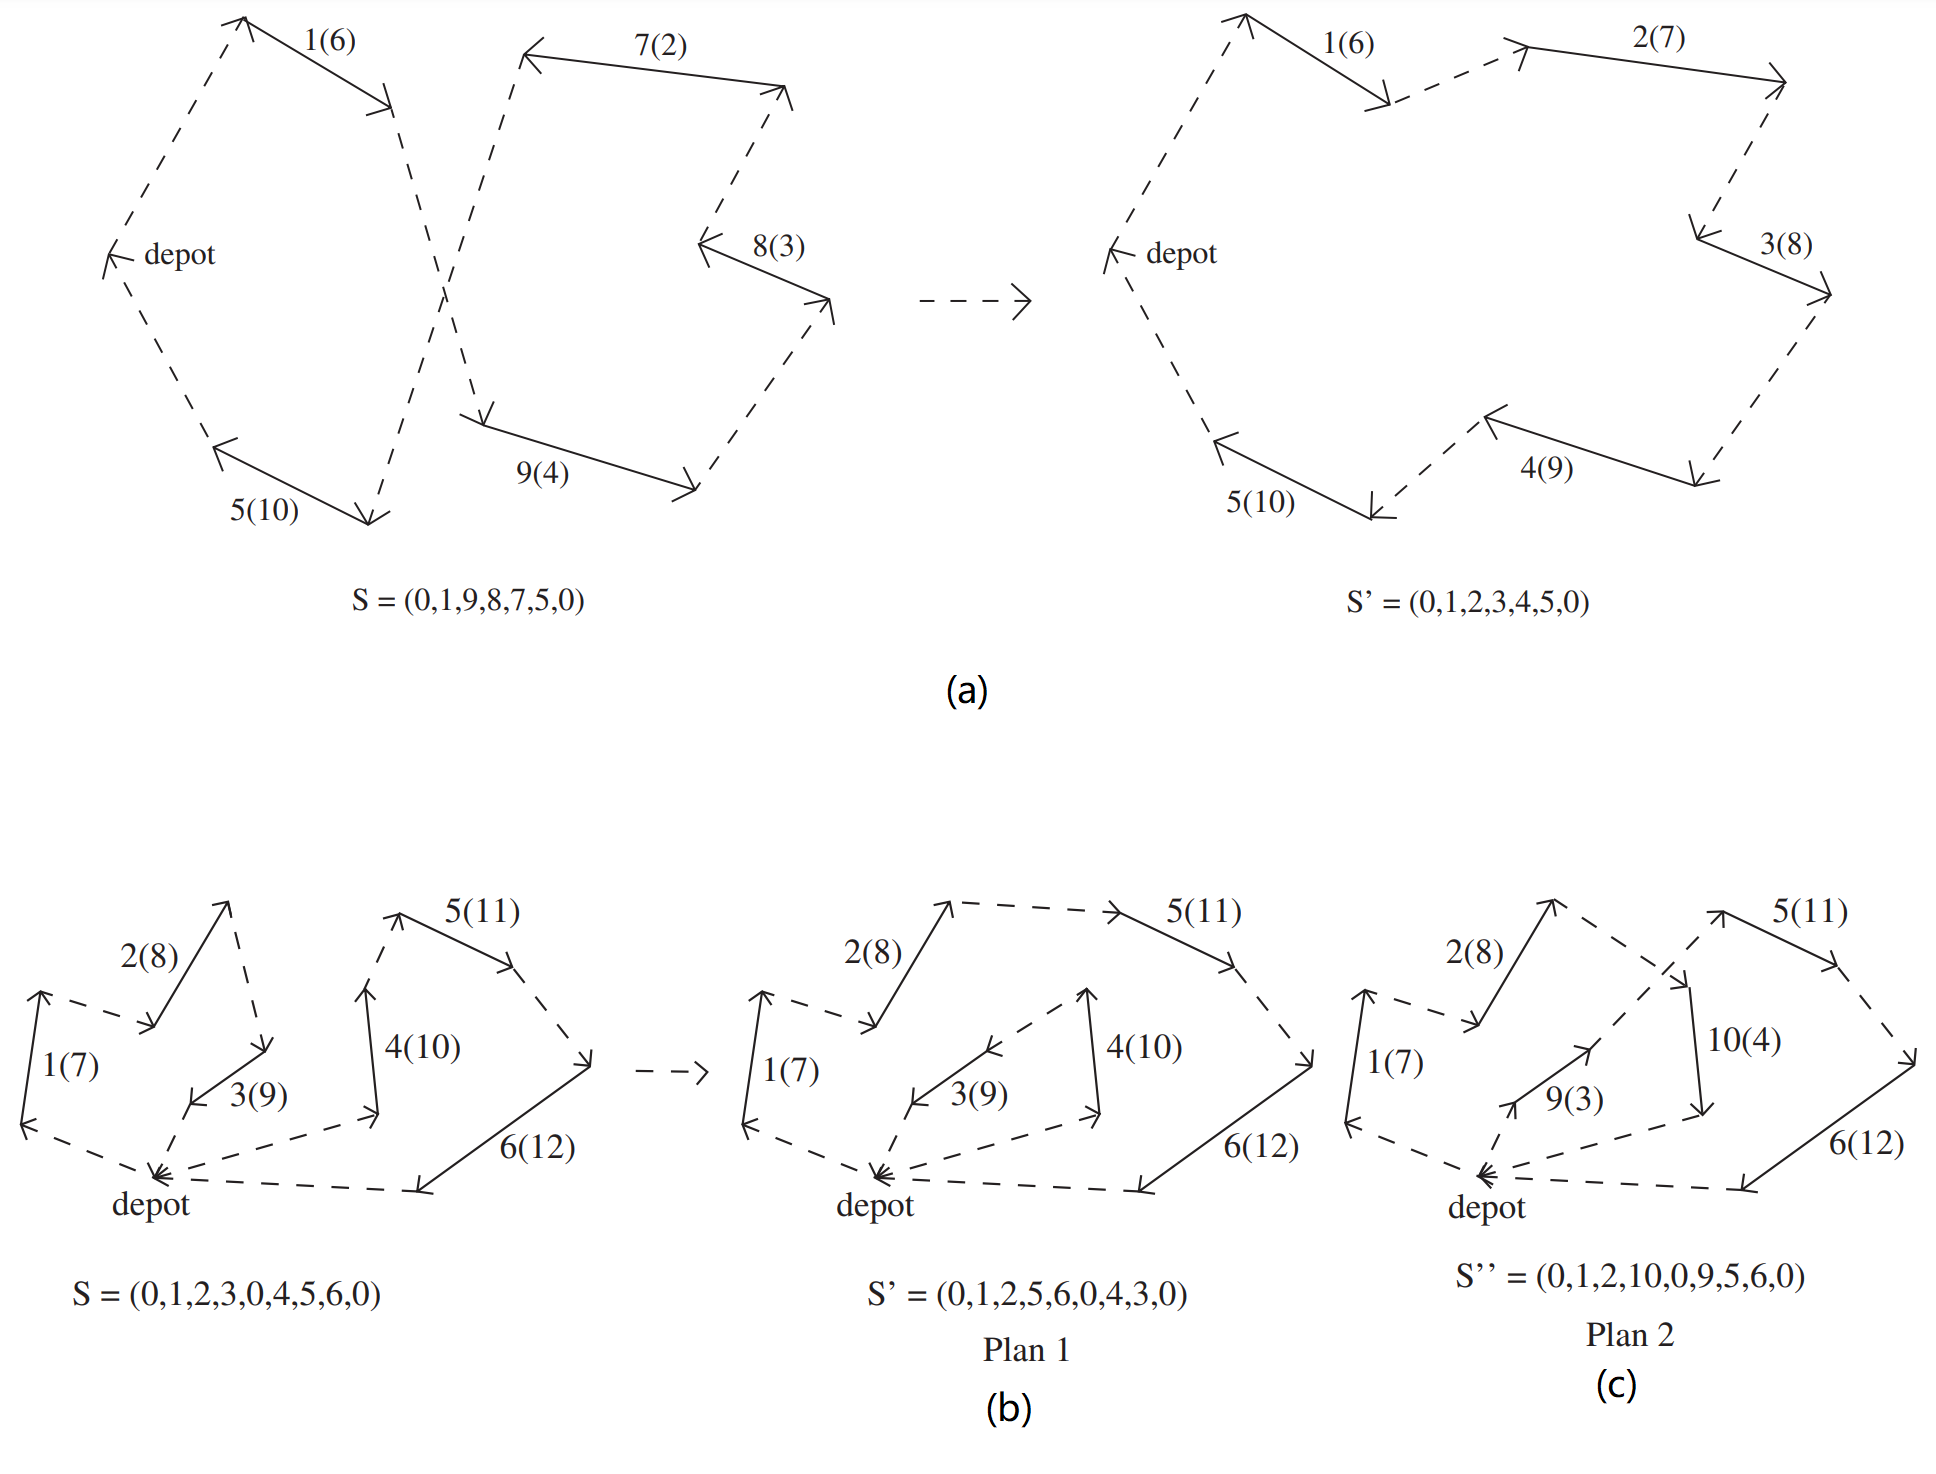
\includegraphics[height=6cm,width=8cm]{fig1.png}
    \caption{Explanation for mutation \textbf{5.$\sim$7.}, cited from\cite{ref2}.}
    \label{fig1}
\end{figure}

Here is the pseudo-code of generating a new population in $O(popsize\times|E|)$ time, assume $\log popsize<<|E|$:

\begin{algorithm}
    \caption{Mutation}
    \KwData{population $p$}
    \KwResult{new population $np$}
    $popsize=p$'s size\;
    $np=p$\;
    \For {individual $i\in p$} {
        \For {each kind of mutation rule} {
            $i'=$ the result of applying the mutation on $i$\;
            \If {$i'$ is valid} {
                $np=np+i'$\;
            }
        }
    }
    $np=$ best $popsize$ individuals in $np$\;
\end{algorithm}

\subsection{Part4. Repeat}

Later, we only need repeat the mutation until the time runs out. In practice, if we detect that the result has not changed for several generations, we can save the best result and back to population initialization, so we will not waste the time.

\subsection{Analysis}

The algorithm above is based on local search model. The first four kinds of mutation method have slighter effects on the solution, while the other three kinds have more remarkable effects. Smaller search steps may trap our agent in local optimal solutions, while bigger search steps may miss local optimal solutions. So we use both kind of methods, which increases our chance to get better solutions.

\section{Experiments}

Environment: CPU: AMD R7 5700X, 3.6GHz

Test data (best result after all optimization):

\resizebox{\linewidth}{!}{
    \begin{center}
        \begin{tabular}{c|c|c|c|c|c}
            Name & Description & 10s result & 60s result & 120s result & 240s result \\ \hline\hline
            egl-s1-A & $|V|=77$ & 6061 & 5548 & 5394 & 5388 \\
            egl-e1-A & $|V|=140$ & 3931 & 3720 & \textbf{3737} & 3630 \\
            gdb1 & $|V|=12,d(e)=1$ & 323 & 316 & 316 & 316 \\
            gdb10 & $|V|=12,d(e)\in\{1,2\}$ & 275 & 275 & 275 & 275 \\
            val1A & $|V|=24$ & 177 & 173 & 173 & 173 \\
            val4A & $|V|=41$ & 460 & 419 & 412 & 408 \\
            val7A & $|V|=40$ & 314 & 291 & 287 & 286 \\
        \end{tabular}
    \end{center}
}

Test data can be seen\cite{ref4}.

We can see an interesting data in the table which I labeled with bold font. The 120s result was worse than the 60s result on the same instance. This indicates our algorithm is not stable enough on larger instances. On the contrary, it performs stably on smaller instances, on which it either keeps optimizing the result or finds the global optimal result in limited time.

During the experiments, I have found many interesting features, for example, in mutation part, instead of storing a hard copy of all demand edges, storing a index array can be far more faster, saving more time for searching, and generating better results. I have also tried multithreading programming and non-fixed $popsize$, but they performed badly.

\section{Conclusion}

In conclusion, my solver makes good use of the running time and generates relatively optimal results in limited time. The result will be worse if we do not generate a new population when evolution ends. Also, I have learned some python programming features in this project, for example, the difference between multithreading and multiprocessing, and the harm of abusing deepcopy.

\begin{thebibliography}{1}
\bibliographystyle{IEEEtran}

\bibitem{ref1}
Y. Nie. {\it{Capacitated Arc Routing Problem}}. \\Available: https://github.com/NYH-Dolphin/SUSTech-Course-Info/blob/main/CS303\%20Articifical\%20Intelligence/Project/Project2-CARP/CARP\%20Report.pdf

\bibitem{ref2}
K. Tang, Y. Mei and X. Yao, "Memetic Algorithm With Extended Neighborhood Search for Capacitated Arc Routing Problems," IEEE Transactions on Evolutionary Computation, vol. 13, (5), 2009. Available: https://www.proquest.com/scholarly-journals/memetic-algorithm-with-extended-neighborhood/docview/875018715/se-2. DOI: https://doi.org/10.1109/TEVC.2009.2023449.

\bibitem{ref3}
Y. Zhao. {\it{CARP Project Steps}}

\bibitem{ref4}

My own github. https://github.com/DeerInForestovo/AIlab/blob/main/project2/CARP/log.txt

\end{thebibliography}

\end{document}


